\chapter{Details of the~method}\label{chap:details}

In this chapter, the~method is described in more detail. Unlike the~previous outline, this description should be sufficient enough for the~reader to implement this method by themselves. In Section~\ref{sec:bottom-top}, it will be said how exactly we construct the~target mip-maps during the~first bottom-top pass and what alternative constructions we also considered. In Section~\ref{sec:top-bottom}, we will explain what is the~form of $\opnorm{P}{}$ - the~prediction operator - and how exactly it is applied in the~second top-bottom pass in order to compute the~residuals needed to reconstruct a~finer mip-map from the~coarser one and also perform the~reconstruction with the~help of these residuals. Note that this method does not use an~update operator, see Chapter~\ref{chap:cbdam_comp} for the~explanation and details.

\section{Bottom-top pass}\label{sec:bottom-top}
As we already said, in the~first bottom-top pass, we just construct the~target mip-maps one by one, from the~largest one - the~input itself - to the~smallest one, sized 1. At each step, we construct a~smaller mip-map from the~last constructed one. The~dimension of the~new mip-map is half the~dimension of the~last one, in other words, it is half as detailed. Generally, we can build the~new mip-map by any form of averaging of pixels of the~larger mip-map. In the~previous chapter, we explained that the~maximum absolute error of the~reconstruction is not dependent on how the~mip-maps look, as long as they contain valid values (no infinities, NaNs). However, the~appearance of the~mip-maps affects the~compression ratio. The~closer the~neighboring mip-maps are to each other, the~lower the~residuals of the~transition from the~smaller one to the~larger one are, thus the~higher the~compression ratio is. Additionally, as described in Chapter~\ref{???}, inside the~renderer in which the~method has been applied, the~mip-maps of a~certain terrain square are carefully selected, so that aliasing is minimized. This decision is based on the~area of the~square projected to the~screen. This means that while looking at a~certain square from above, its finest mip-map is displayed and during a~fixed-radius circular traversal around it up to the~point when we look at it from a~side, we will be gradually displaying coarser (less detailed) mip-maps of the~square. This means that if the~mip-maps are significantly different from each other, disturbing visual artifacts might occur during this traversal. The~best way how to minimize these artifacts is to use the~simplest form of averaging of heights when producing a~lower-resolution mip-map where the~height at every pixel of the~smaller mip-map $\lnorm{i}$ will be the~average of the~heights of the~four corresponding neighboring pixels inside the~larger mip-map $\lnorm{i+1}$:

\begin{equation}
\label{eq:averaging}
\lnorm{i}[m][n] = \frac{\sum\limits_{om=0}^{1}\sum\limits_{on=0}^{1}\lnorm{i+1}[2m + om][2n + on]}{4}
\end{equation}

For a~comparison, in transition to a~coarser LOD in C-BDAM, a~different form of heights averaging is utilized. It properly conforms to the~standard lifting scheme - it uses the~update operator to produce the~coarser LOD.  This averaging is even parametrized by one coeffiecient named subsampling weight the~value of which can span from 0 to 1. To the~contrary, our method does not use the~update operator there which is explained in Chapter~\ref{chap:cbdam_comp}. However, we tried to use a~similar averaging of pixels inspired by the~one performed in the~update operator in C-BDAM. With the~subsampling weight well set, we achieved a~slightly better compression ratio, but the~mentioned visual artifacts were more disturbing. At last, we decided to minimize the~visual artifacts, as they really affect the~user experience, and stick to the~described simple averaging (eq.~\ref{eq:averaging}).

\section{Top-bottom pass}\label{sec:top-bottom}
This pass is performed in the~offline compression after the~first bottom-top pass, in which case it computes the~residuals $\objdot{E}{0..n}$ needed to completely progressively reconstruct the~compressed multiresolution representation of the~input $\lnorm{n}$. During the~following real-time decompression, this is the~only pass which is performed, with the~only difference that it no longer computes the~residuals, but it just reads them and uses them to reconstruct the~data. Let us describe it detailly, so that it becomes clear how this pass is implemented.

In the~previous chapter describing the~outline of the~method, we claimed that we construct a~larger compressed mip-map $\ldot{i+1}$ from the~smaller $\ldot{i}$ in just one step (eq.~\ref{eq:nextLevel}). This is not exacly true, it is a~simplification which we made for several reasons: to give the~reader a~simple high-level idea of the~method, to make the~fact that $maxdev(\ldot{i+1}, \lnorm{i+1}) < \objnorm{D}{}$ easier to see and to make it clear that the~way the~target mip-maps $\lnorm{n-1..0}$ look has no effect on this constraint. However, the~truth is that to get $\ldot{i+1}$ from $\ldot{i}$, the~prediction operator $\opnorm{P}{}$ is applied consecutively three times. Its form is different at each of these applications which reflects the~fact that before each application, different height values are known - the~later the~application, the~more values are known. After each of these applications, the~residuals are computed during the~compression and added to~the already computed values during both the~compression and decompression. Nevertheless, the~two main principles which ensure that the~maximum error bound between $\lnorm{i+1}$ and $\ldot{i+1}$ is kept remain unchanged - during the~compression, the~residuals are still computed against the~target mip-map $\lnorm{i+1}$ after each application of $\opnorm{P}{}$ and all predictions are made from the~compressed values which ensures that both the~compression and the~decompression add the~residuals to the~same values. Hence, let us explain how these three steps are performed.

 When constructing the~larger compressed mip-map $\ldot{i+1}$ from $\ldot{i}$, we can imagine it as every pixel $p$ from $\ldot{i}$ being substituted by four pixels $a, b, c, d$ in $\ldot{i+1}$ as depicted in Fig.~\ref{fig:subst}. This substitution is the~exact inverse of the~one performed in the~first bottom-top pass described in the~previous section ???. We will apply the~prediction operator and subsequent residuals computation and addition three times in order to compute the~values of the~four pixels and the~residuals needed to reconstruct them from $p$ during the~decompression.

\begin{figure}
	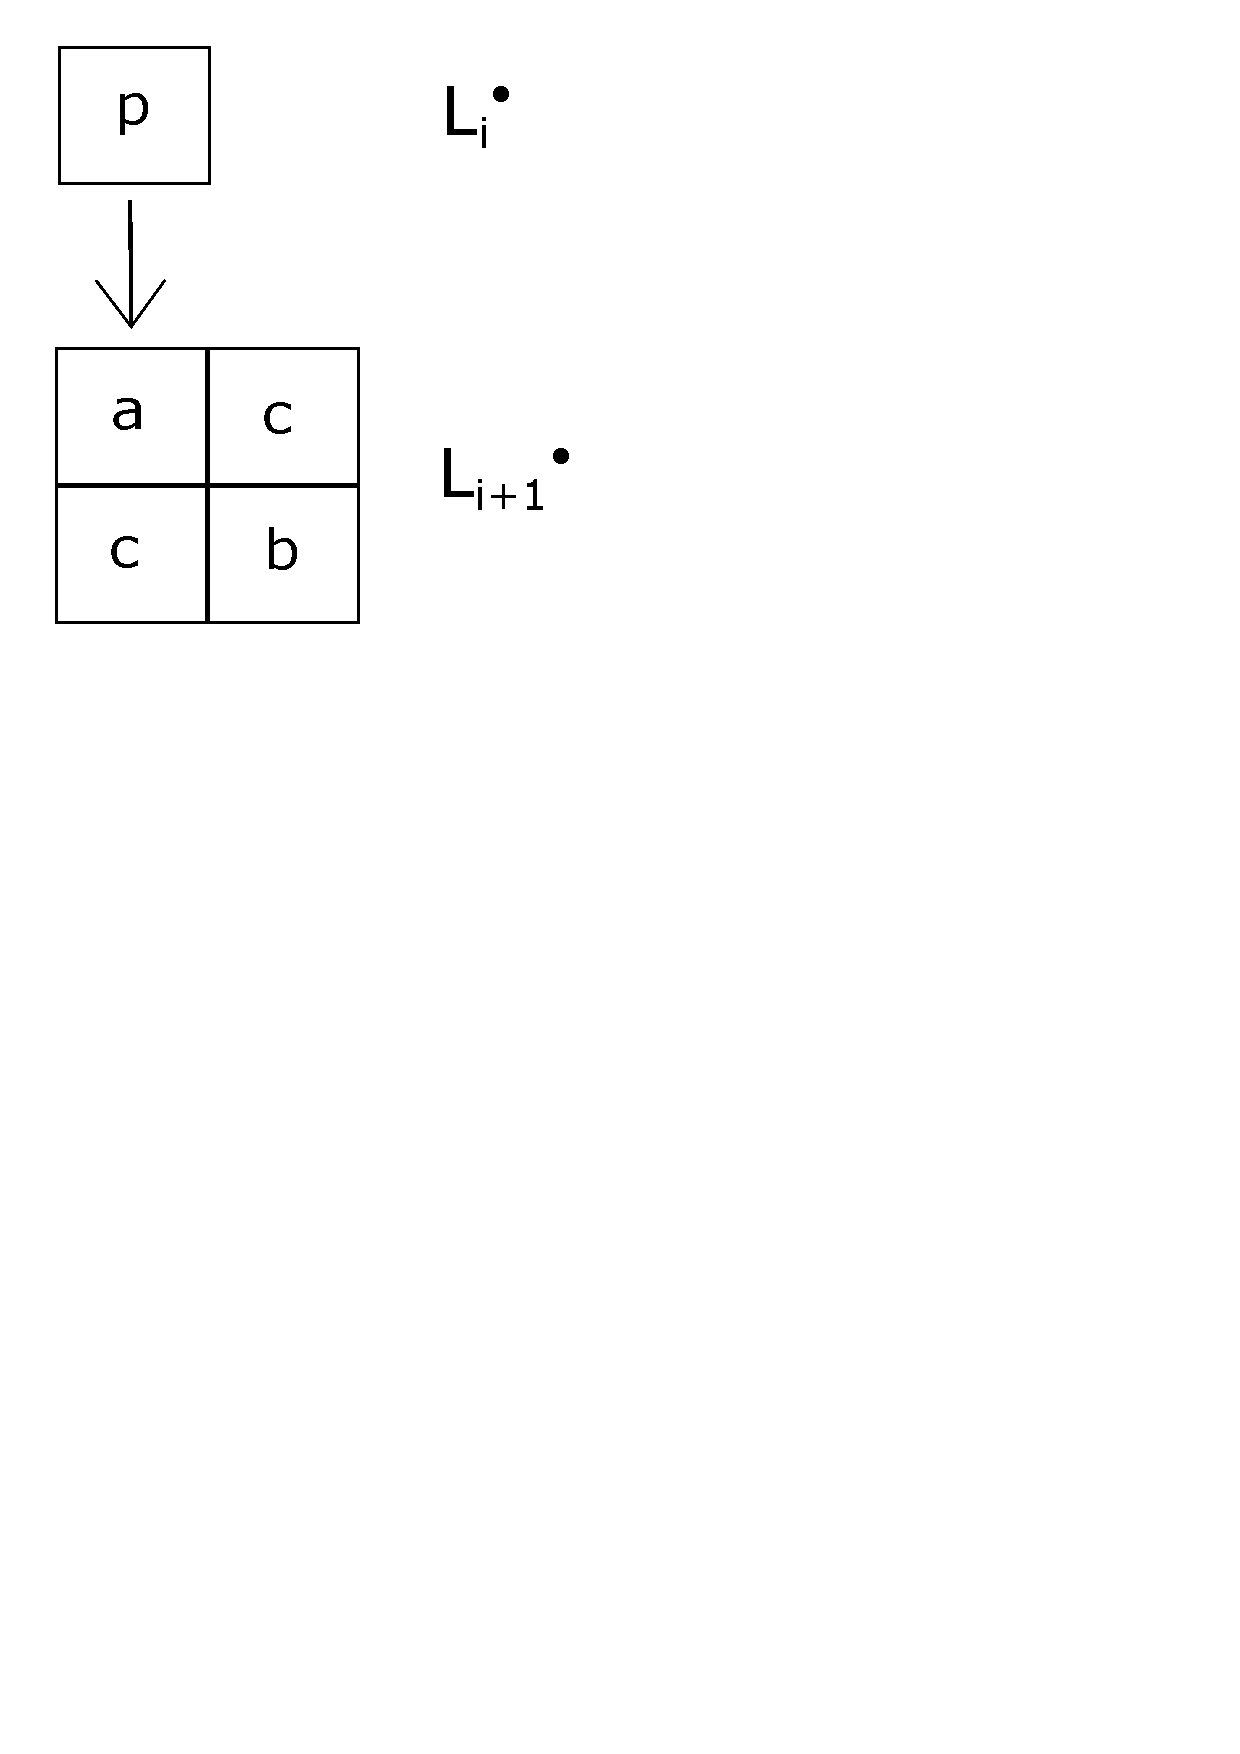
\includegraphics[trim={0 19cm 11cm 0}, clip, width=0.28\textwidth]{figures/subst.pdf}\centering
	\caption{Substituting the~pixel p in $\ldot{i}$ with four pixels in $\ldot{i+1}$}
	\label{fig:subst}
\end{figure}
In the~first of the~three steps, we compute the~pixels labeled $a$. To predict them from their corresponding $p$ pixels inside $\ldot{i}$, we use a~simple prediction operator $\opnorm{P}{a}(\ldot{i}) = p$. We compute the~residuals $\objnorm{E}{a}$ and $\objdot{E}{a}$ with respect to the~target value $a_t$ in $\lnorm{i+1}$ and then assign $a$ the~final value $a\bullet$ (eq. \ref{eq:a}, recall that $\opnorm{Q}{D}$ is a~uniform quantizer respecting the~maximum deviation $D$: $maxdev(v, \opnorm{Q}{D}(v)) < D$. It is clear that  $maxdev(a\bullet, a_{t}) \leq \objnorm{D}{}$. The~explanation would be the~same as in Chapter~\ref{chap:outline}.

$$\objnorm{E}{a} = a_t - p$$
$$\objdot{E}{a} = \opnorm{Q}{D}(\objnorm{E}{a})$$
\begin{equation}
\label{eq:a}
a\bullet = p + \objdot{E}{a}
\end{equation}

In the~second of the~three steps, we compute the~pixels labeled $b$. We do not predict them from $\ldot{i}$ anymore, but from the~already available pixels $a\bullet$ inside $\ldot{i+1}$. The~prediction operator $\opnorm{P}{b}$ used for this has now the~form of a~straight-oriented Neville interpolating filter of order 2. All it does is that when it is requested to predict the~height at some pixel, it just averages the~heights of its certain four neighboring pixels as depicted in Fig.~\ref{fig:bcomp}. It is easy to see that as long as it is requested to predict the~height at pixels $b$, it always averages only the~already known $a\bullet$ pixels. This is the~same prediction operator as the~one used in C-BDAM to predict the~heights of the~samples located at the~border of a~LOD hierarchy node. Once the~predictions of $b$ pixels are known, we perform an~analogic computation of residuals $\objnorm{E}{b}$ and their quantizations $\objdot{E}{b}$, again with respect to the~corresponding target values $b_t$ in $\lnorm{i+1}$. Finally, we assign $b$ its final value $b\bullet$ (eq.~\ref{eq:b}).

\begin{figure}
	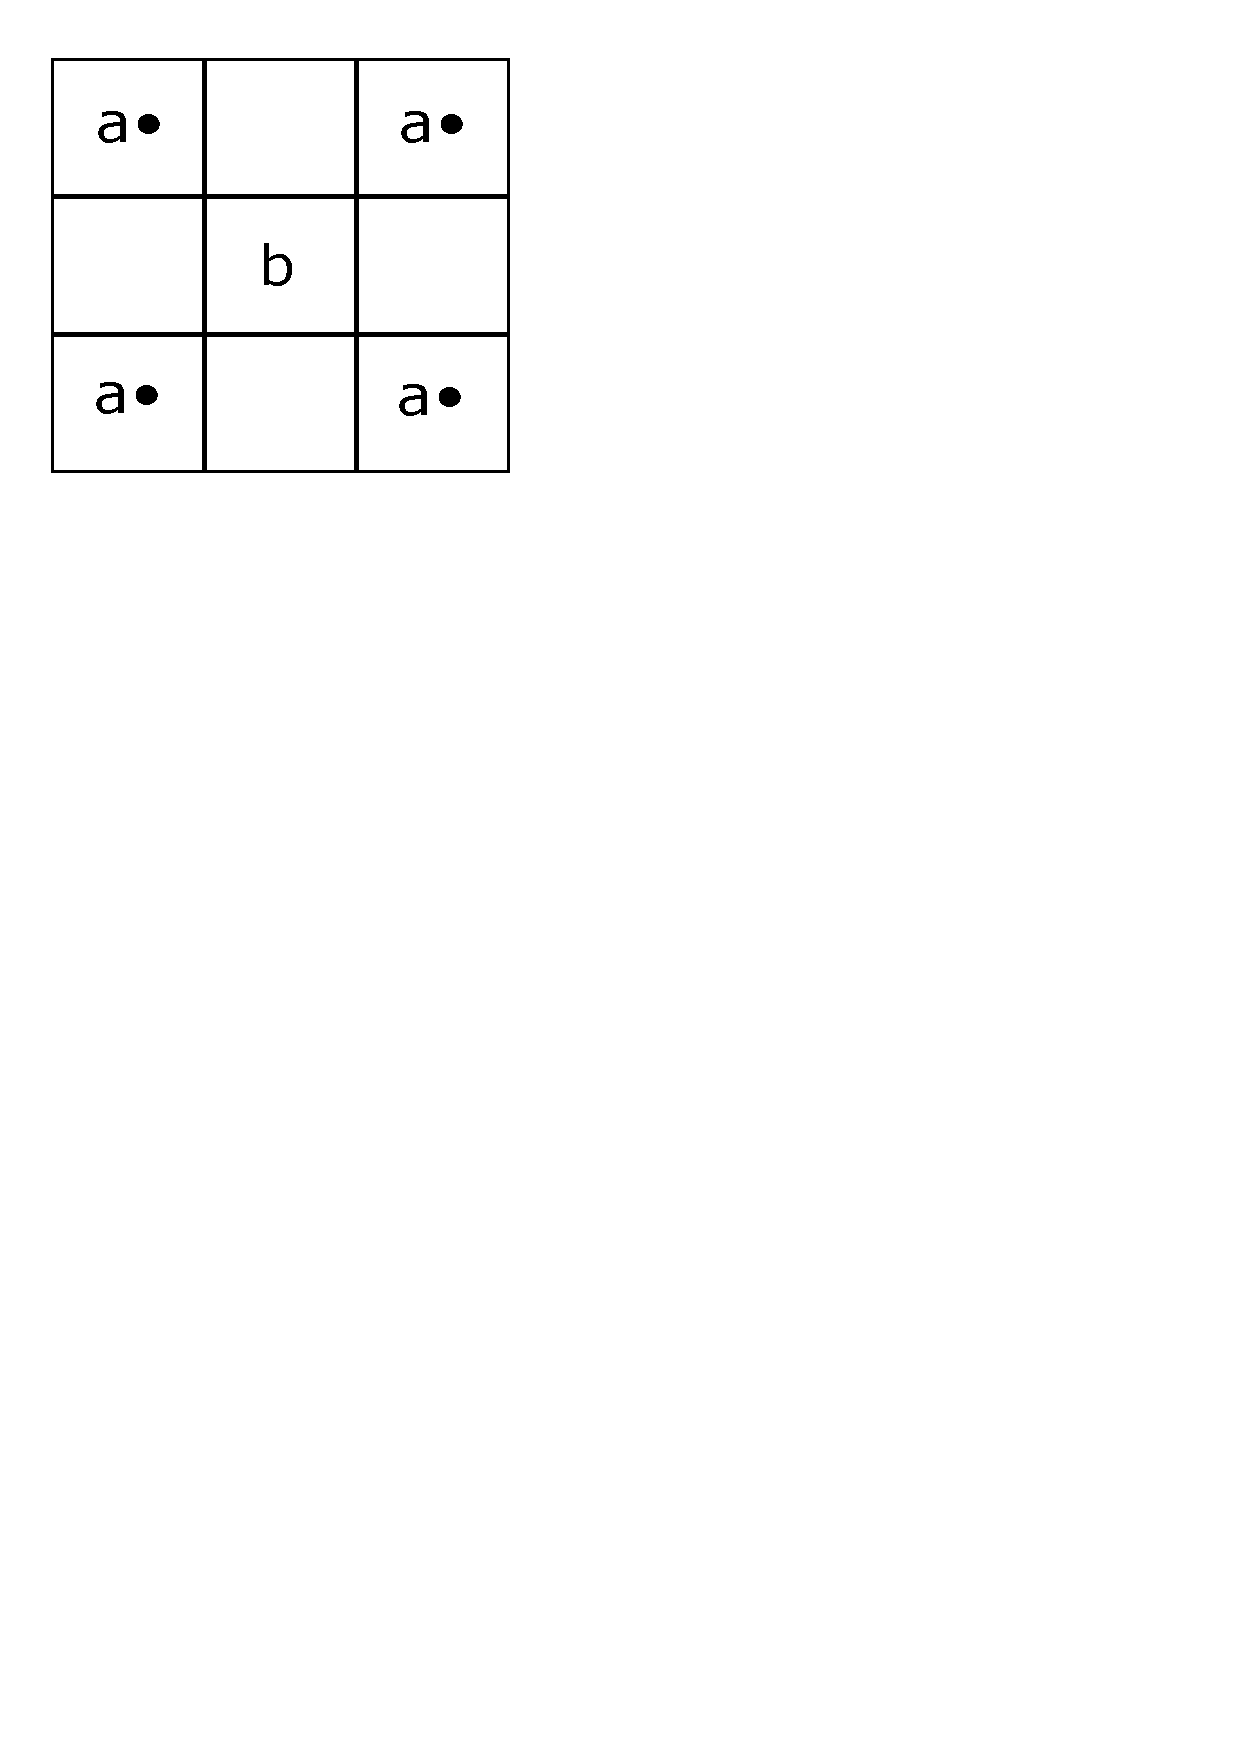
\includegraphics[trim={0 21cm 10cm 0}, clip, width=0.3\textwidth]{figures/bcomp.pdf}\centering
	\caption{The~prediction of $b$ - $\opnorm{P}{b}(\ldot{i+1})$ - is the~average of all the~displayed $a\bullet$}
	\label{fig:bcomp}
\end{figure}

$$\objnorm{E}{b} = b_t - \opnorm{P}{b}(\ldot{i+1})$$
$$\objdot{E}{b} = \opnorm{Q}{D}(\objnorm{E}{b})$$
\begin{equation}
\label{eq:b}
b\bullet = \opnorm{P}{b}(\ldot{i+1}) + \objdot{E}{b}
\end{equation}

The~reason why C-BDAM uses the~order 2 Neville interpolating filter at the~borders is that thanks to the~way the~samples are organized inside a~node of its LOD hierarchy, the~filter does not pick the~samples behind the~node's border. We can view the~mip-map in our method as an analogy to the~node in C-BDAM. However, the~spatial organization of mip-map samples in our method differs from the~organization of samples inside a~LOD node in C-BDAM, so unlike in C-BDAM, in our method it might happen that this interpolating filter comes out of the~underlying mip-map. We handle this by only including the~valid interior values in the~resulting average and completely ignoring the~imaginary values behind the~mip-map borders. Thus, when computing a~certain prediction, we count how many times the~filter has hit the~interior of mip-map and divide the~sum of the~valid interior heights with this number of hits. Most of the~times, the~number of hits will be 4, but it will be 2 at the~borders and just 1 at the~corners. This way, it is always ensured that the~filter does not make any data up, unlike the~possible alternative of some mirror extension of data behind the~borders. ??? Comparison with mirror extension ???

C-BDAM uses the~larger order 4 Neville interpolating filter to predict the~heights at the~interior of a~node of its LOD hierarchy. This filter covers larger area - it samples twelve points instead of four. In addition, it does not compute the~average of these points, but their weighted sum. Just like in the~case of simple averaging, the~sum of the~weights is 1. The~difference is that the~four closest points have a~certain positive weight, whereas the~remaining eight further points have a~different negative weight, the~absolute value of which is lower than the~first weight (Fig.~???). The~property with the~lower absolute value indicates that the~points which are further affect the~result less. The~fact that their weights are negative basically means that the~valleys and hills are predicted better (Fig.~???). 

Unlike C-BDAM, this method uses the~smaller order 2 filter even for the~interior samples. Let us explain the~reasons why we decided to do so. The~first reason is the~increase of speed. The~order 2 filter only averages four values, whereas the~order 4 filter averages 12 values. Moreover, the~subsequent averaging performed by the~order 2 filter can easily be cached during the~horizontal traversal which is an~additional reduction of the~computation overhead (Fig.~???). We also tried using the~order 4 filter with various weights settings for the~interior values, too. This slightly increased the~compression ratio - probably because this~filter is better at predicting hills and walleys - but worsened the~quality of compression by producing more significant artifacts near smooth terrain's borders (Fig.~\ref{fig:artifs_border}) and sharp terrain transitions (Fig.~\ref{fig:artifs_sharp_change}). The~most probable cause of this is that the~predictions made by the~order 4 filter tend to differ from the~neighboring heights more. This emphasises the~artifacts.

\newcommand{\incimg}[3]{\includegraphics[width=#1px, height=#2px]{#3}}
\newcommand{\incartifborder}[1]{\incimg{95}{70}{#1}}

\begin{figure}
	Original \incartifborder{figures/artif_orig0.png}
	\incartifborder{figures/artif_orig1.png}\\
	Order 2~~\incartifborder{figures/artif_four0.png}
	\incartifborder{figures/artif_four1.png}\\
	Order 4~~\incartifborder{figures/artif_twelve0.png}
	\incartifborder{figures/artif_twelve1.png}\\
	\caption{Two examples of the~difference between artifacts caused by order 2 and order 4 filters near smooth terrain's border - in the~first row there are the~target heightmaps, in the~second, there are the~same heightmaps compressed using the~order 2 filter, in the~third row, the~heightmaps compressed with the~order 4 filter.}
	\label{fig:artifs_border}
\end{figure}

\newcommand{\incartifchange}[1]{\incimg{95}{95}{#1}}

\begin{figure}
	Original \incartifchange{figures/artif_change_orig0.png}
	\incartifchange{figures/artif_change_orig1.png}\\
	Order 2~~\incartifchange{figures/artif_change_four0.png}
	\incartifchange{figures/artif_change_four1.png}\\\
	Order 4~~\incartifchange{figures/artif_change_twelve0.png}
	\incartifchange{figures/artif_change_twelve1.png}\\
	\caption{Two examples of the~difference between artifacts caused by order 2 and order 4 filters near a~sharp terrain change - in the~first row there are the~target heightmaps, in the~second row, the~same heightmaps compressed using the~order 2 filter, in the~third row, the~heightmaps compressed with the~order 4 filter. The~span of the~values in the~original images is from 0 to 16 and the~maximum absolute deviation ($D$) of compression is set to 9.}
	\label{fig:artifs_sharp_change}
\end{figure}

Generally, the~reason why these artifacts occur is that as long as the~predictions are close enough to the~target mip-map and their quantized residuals are equal to zero, the~compressed values might remain above/under the~terrain for a~long time, but only until one prediction gets a~bit further from the~target terrain. As soon as it happens, its associated residual will be quantized to a~certain non-zero value which will result in the~reconstructed value being flipped to the~opposite side of the~real terrain which produces a~visual artifact. It is not a~coincidence that this often occurs near a~sharp change in the~terrain. The~predictions produced by the~averaging filter get a~bit different from the~adjacent ones near this change, because at these places, the~filter reaches out to the~area behind the~change (Fig.~\ref{fig:artifs_theory2}, \ref{fig:artifs_theory}). This difference might then cause the difference in residuals - the~quantized residuals further from this change might be all zeroes, whereas the~residual near this change not, causing a~spike to occur. This spike will then get propagated to the~following compressed mip-map levels. The~only thing that is guaranteed is that the~maximum error bound is still satisfied. ???(musim overit, clipping je nasadeny len v Bohemke, ale je to lepsi napad ako mirroring, tusim, ze to aj zlepsilo kompresny pomer, no nezistoval som pri nom, ake su artefakty)The~clipping performed by the~predicting filter near the~mip-map borders creates the~effect similar to a~sharp terrain change, too, in a~bit different way - by the~sole fact that the~terrain behind the~border no longer follows its trend up to the~border (rising, for example), but is practically mirrored behind the~border (following the~example, falling), because instead of reaching out to the~non-existing values out of the~mip-map, the~existing ones are used.???

(potial iba)

\begin{figure}
	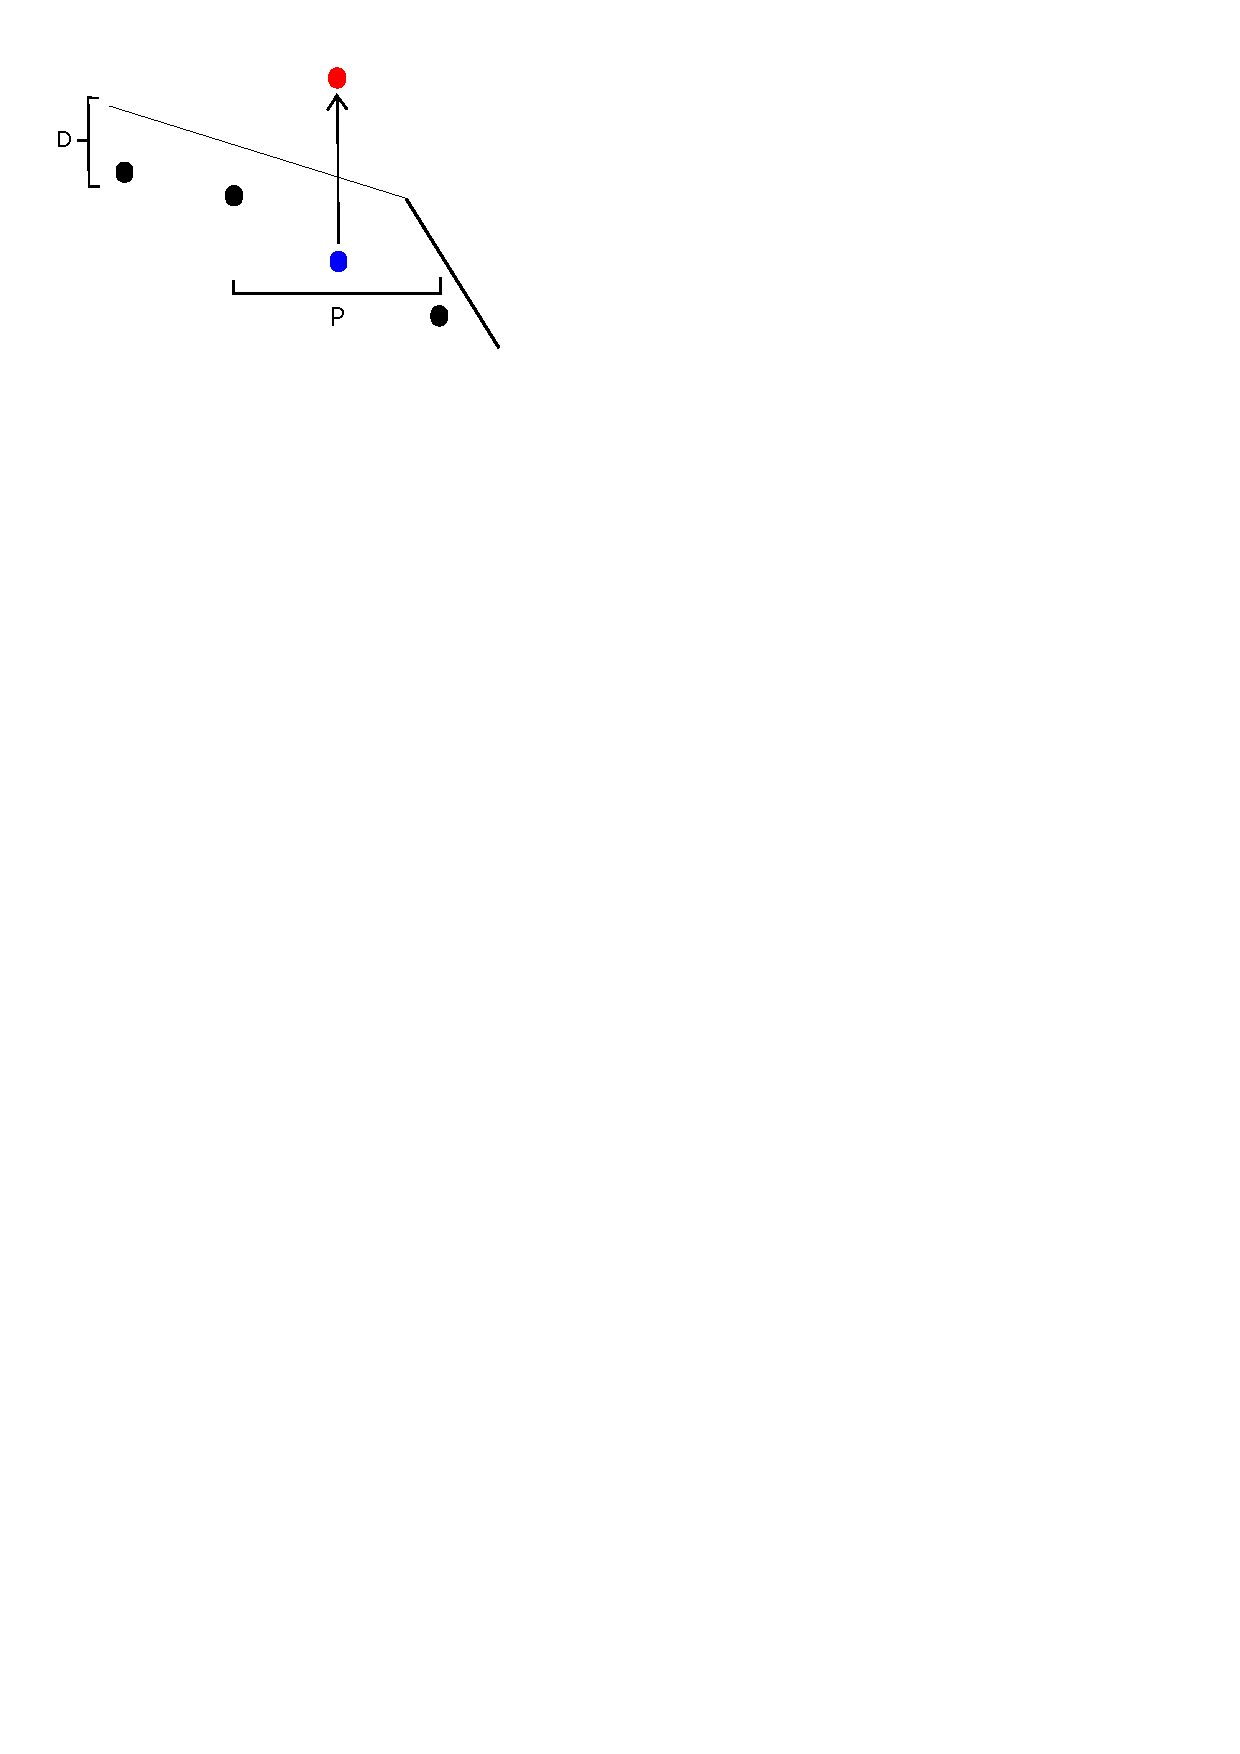
\includegraphics[trim={0 24cm 7cm 0}, clip, width=0.45\textwidth]{figures/artifs_theory.pdf}\centering
	\caption{The~illustration of how an~artifact occurs - the~black predictions are within the~maximum-error bound $D$, so they are equal to the~reconstructed values, but the~blue one is not. Because a~uniform quantizer is used, the~blue prediction is shifted by $2D - 1$ to the~top, creating an~artifact.}
	\label{fig:artifs_theory2}
\end{figure}

\begin{figure}
	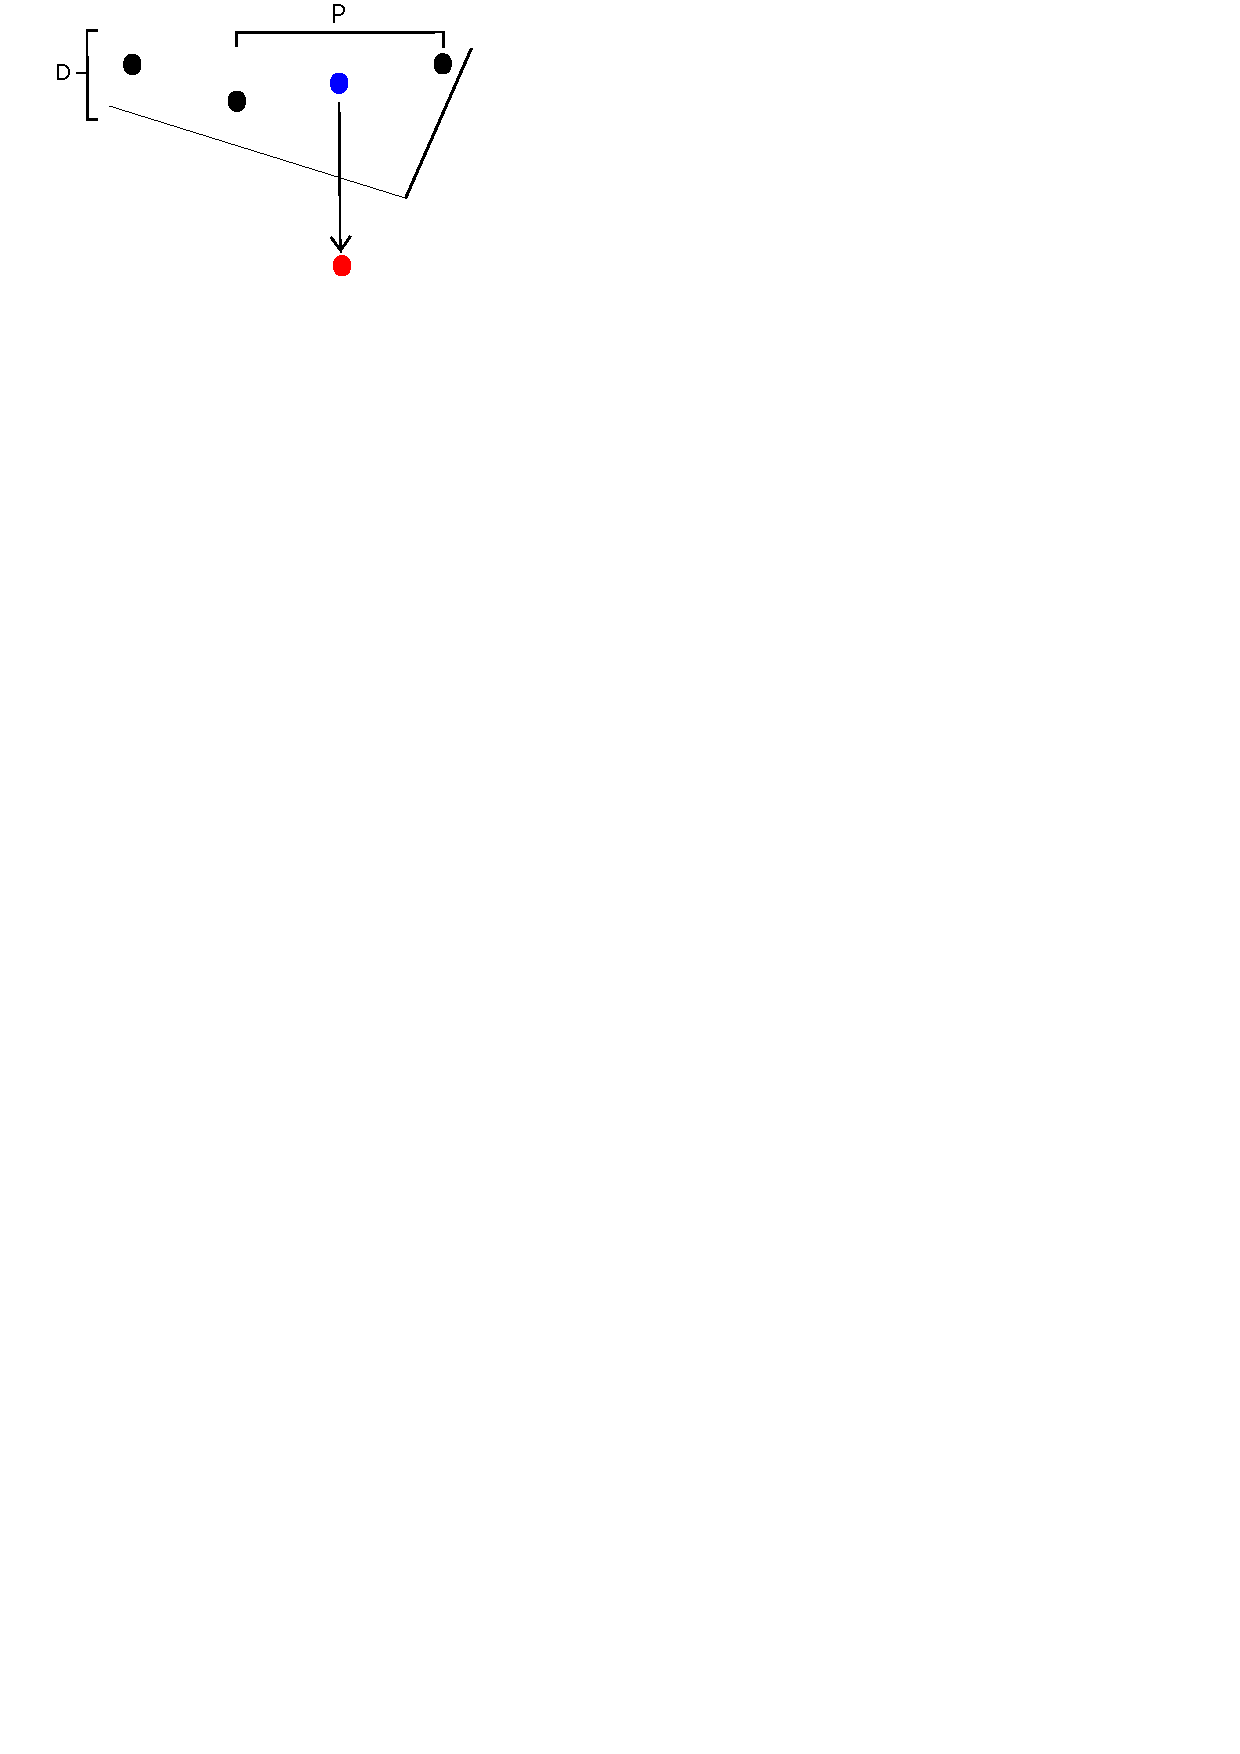
\includegraphics[trim={0 24cm 7cm 0}, clip, width=0.45\textwidth]{figures/artifs_theory2.pdf}\centering
	\caption{Another~illustration of an~artifact - the~black predictions are within the~maximum-error bound $D$, but the~blue one is not. The~blue prediction is shifted by $2D - 1$ to the~bottom, creating an~artifact.}
	\label{fig:artifs_theory}
\end{figure}

The~remaining pixels labeled $c$ are predicted from the~pixels $a\bullet$ and $b\bullet$ in $\ldot{i+1}$ by the~diagonally-oriented order 2 Neville interpolating filter (fig. \ref{fig:ccomp}). The~computation of residuals $\objnorm{E}{c}$ and $\objdot{E}{c}$ then follows according to the~target value $c_t$ from $\lnorm{i+1}$ and $c$ is assigned the~final value $c\bullet$ (eq. \ref{eq:b}).

\begin{figure}
	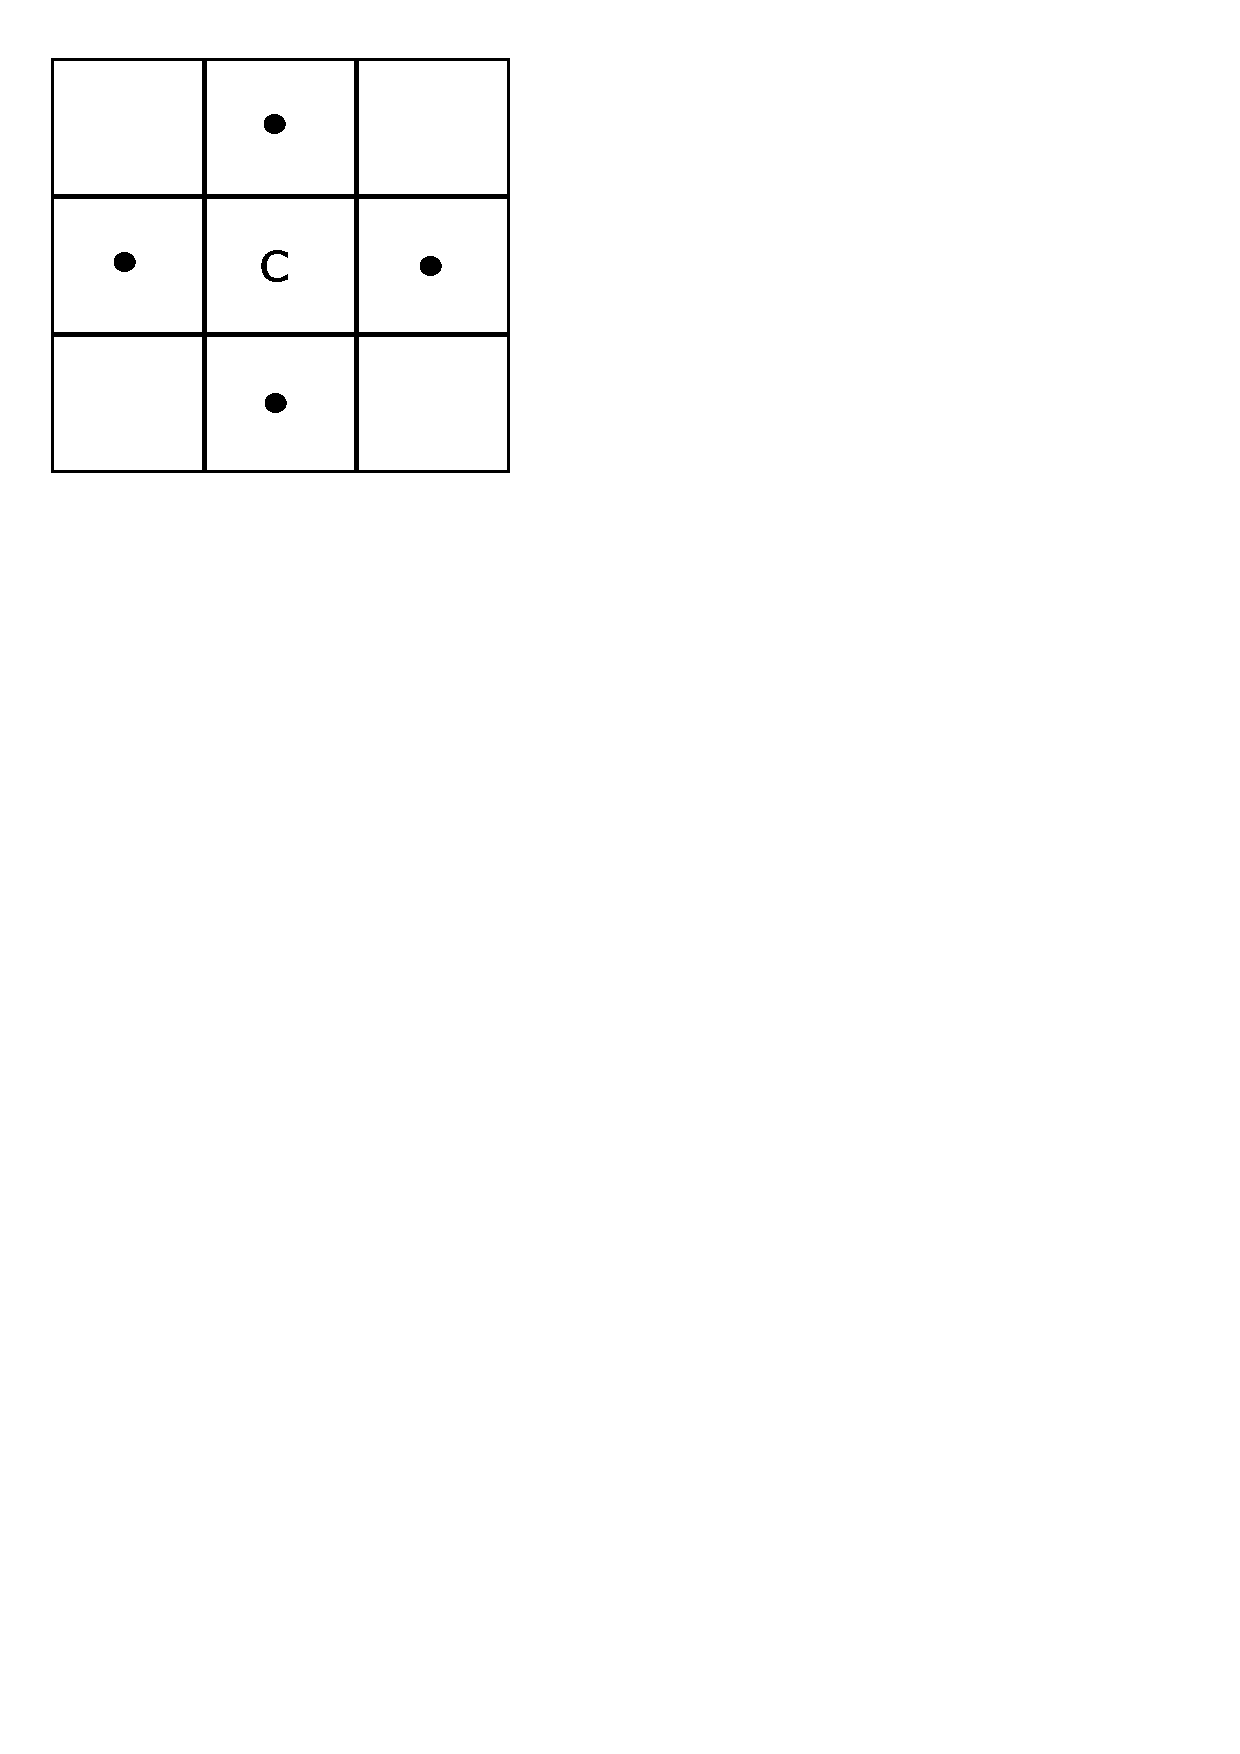
\includegraphics[trim={0 21cm 10cm 0}, clip, width=0.3\textwidth]{figures/ccomp.pdf}\centering
	\caption{The~prediction of $c$ - $\opnorm{P}{c}(\ldot{i+1})$ - is the~average of all the~pixels marked with a~dot - $\bullet$.}
	\label{fig:ccomp}
\end{figure}

$$\objnorm{E}{c} = c_t - \opnorm{P}{c}(\ldot{i+1})$$
$$\objdot{E}{c} = \opnorm{Q}{D}(\objnorm{E}{c})$$
\begin{equation}
\label{eq:c}
c\bullet = \opnorm{P}{c}(\ldot{i+1}) + \objdot{E}{c}
\end{equation}

The~cases when the~filter comes out of the~image are handled by a~specific mirror extension (fig. \ref{fig:cborders}). For the~same reasons as in the~prediction of $b$ pixels, the~order 2 filter is used for the~prediction of all $c$ pixels - both interior and exterior ones. Similarly, the~interpolation with such filter can be cached during diagonal traversal.

The~residuals $\objdot{E}{a}$, $\objdot{E}{b}$ and $\objdot{E}{c}$ are then encoded by an~entropy codec and stored. The~decompression is done in a~similar manner with the~only difference that the~residuals  are not computed anymore, but just decoded and read. So, we substitute every pixel from $\ldot{i}$ by four pixels in $\ldot{i+1}$, the~value of which is computed in three passes of prediction followed by adding the~read residual (the~last lines of eq. \ref{eq:a}, \ref{eq:b}, \ref{eq:c}).

\begin{figure}
	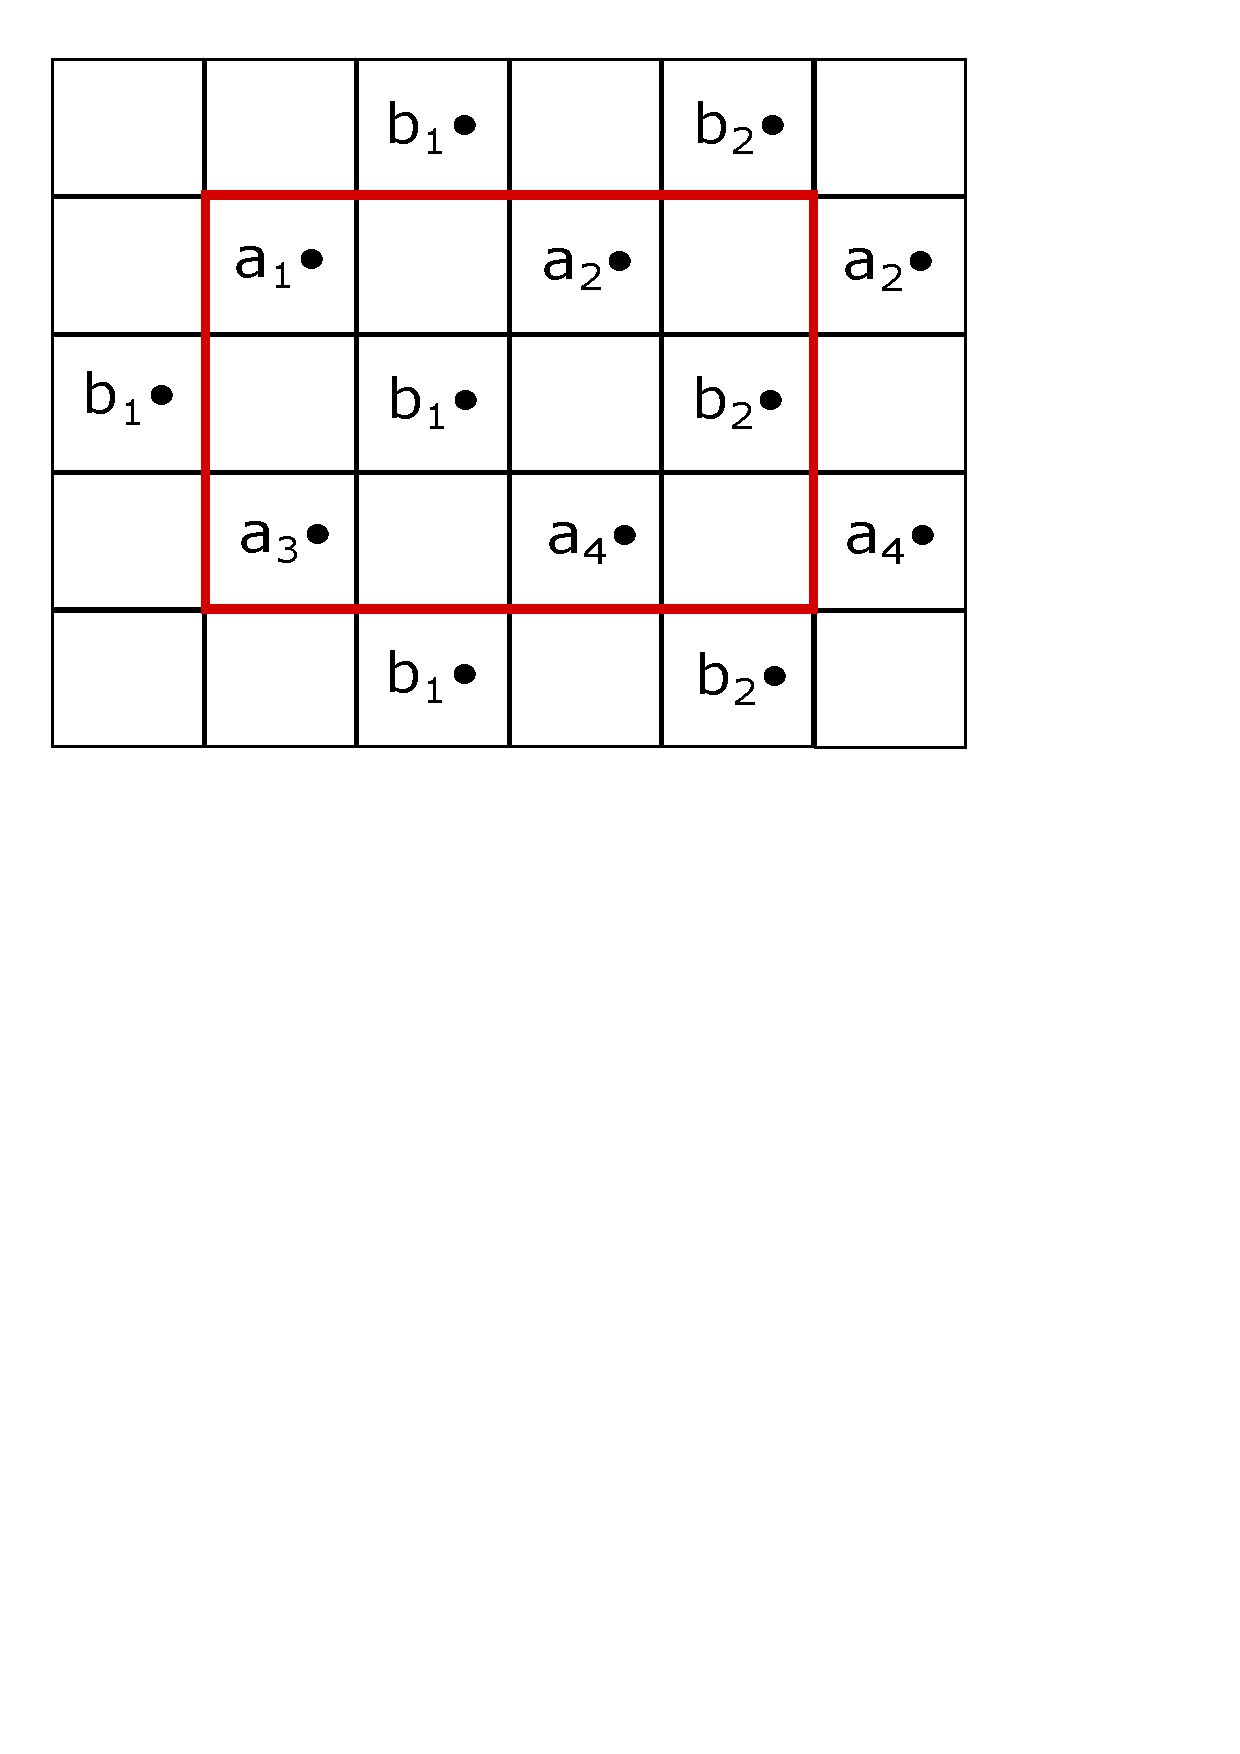
\includegraphics[trim={0 17cm 3cm 0}, clip, width=0.45\textwidth]{figures/extc.pdf}\centering
	\caption{Handling of border cases in the~computation of $\opnorm{P}{c}(\ldot{i+1})$ - the~red line represents the~border.}
	\label{fig:cborders}
\end{figure}